\documentclass[twocolumn, 10pt]{article}
\usepackage[utf8]{inputenc}
\usepackage[margin=15mm]{geometry}
\usepackage{amsmath, amssymb}
\usepackage{tikz}
\usepackage{chemfig}
\usepackage{chemformula}
\usepackage{enumitem}
\usepackage{graphicx}

\title{2024 U.S. National Chemistry Olympiad\\National Exam Part I}
\date{}
\author{}

\setlist[enumerate]{leftmargin=*}

\begin{document}

\maketitle

\section*{Directions}
Each item in Part I consists of a question or an incomplete statement followed by four possible choices. Select the single choice that best answers the question or completes the statement.

\begin{enumerate}

    \item What is the mole fraction of acetic acid (\ch{CH3COOH}, $M = 60.05$) in an aqueous solution that is 11.7\% by mass acetic acid?
    \begin{enumerate}
        \item 0.00195
        \item 0.0382
        \item 0.0398
        \item 0.195
    \end{enumerate}

    \item Hydrogen peroxide ($M = 34.02$) decomposes to give water and oxygen gas. How much 3.00\% by mass aqueous \ch{H2O2} must decompose to afford 4.00 L of dry \ch{O2} at STP?
    \begin{enumerate}
        \item 6.08 g
        \item 101 g
        \item 203 g
        \item 405 g
    \end{enumerate}

    \item A diamagnetic compound that contains only carbon, hydrogen, nitrogen, and oxygen is 19.99\% C, 3.35\% H, and 23.31\% N by mass. Which is its molecular formula?
    \begin{enumerate}
        \item \ch{CH2N2O}
        \item \ch{CH2NO2}
        \item \ch{C2H3NO}
        \item \ch{C2H4N2O4}
    \end{enumerate}

    \item What is the chloride ion concentration in a solution prepared by mixing 35.0 mL of 0.35 M sodium chloride and 65.0 mL of 0.65 M calcium chloride?
    \begin{enumerate}
        \item 0.50 M
        \item 0.54 M
        \item 0.85 M
        \item 0.97 M
    \end{enumerate}

    \item 17.0 g \ch{Ba(NO3)2} ($M = 261.32$) is mixed with 11.5 g of an alkali metal sulfate and the precipitated \ch{BaSO4} ($M = 233.37$) is collected by filtration, placed in a tared crucible, and the crucible heated to drive off water. The mass of \ch{BaSO4} obtained is 15.4 g. Which conclusion is best supported by the data?
    \begin{enumerate}
        \item The sulfate salt used was \ch{Na2SO4} ($M = 142.04$).
        \item The sulfate salt used was \ch{K2SO4} ($M = 174.26$).
        \item The \ch{BaSO4} was not heated long enough to drive off all the water.
        \item Some of the \ch{BaSO4} was spilled before it was transferred to the crucible.
    \end{enumerate}

    \item 10.0 mL of 0.50 M potassium sulfate and 10.0 mL of 0.50 M silver nitrate solutions are mixed and the mixture is allowed to attain equilibrium. Which ordering of the concentrations of the ions in solution is correct?
    \begin{enumerate}
        \item $[\ch{K+}] = [\ch{NO3-}] > [\ch{Ag+}] > [\ch{SO4^2-}]$
        \item $[\ch{K+}] = [\ch{NO3-}] > [\ch{SO4^2-}] > [\ch{Ag+}]$
        \item $[\ch{K+}] > [\ch{NO3-}] > [\ch{Ag+}] > [\ch{SO4^2-}]$
        \item $[\ch{K+}] > [\ch{NO3-}] > [\ch{SO4^2-}] > [\ch{Ag+}]$
    \end{enumerate}

    \item A neutral organic compound is to be separated from a basic impurity by washing a solution of the compound in hexane with 5\% aqueous \ch{HCl}. Which apparatus is best suited to this operation?
    
    \begin{center}
    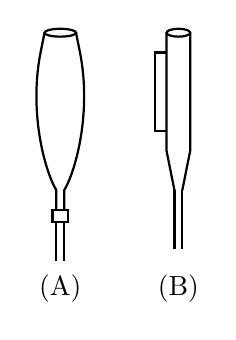
\begin{tikzpicture}[scale=0.5]
        % (A) Separatory Funnel
        \draw[thick] (0,3) ellipse (0.4 and 0.1);
        \draw[thick] (-0.4,3) -- (-0.5,2.5) .. controls (-0.8,1) and (-0.4,-0.5) .. (-0.1,-1) -- (-0.1,-1.5);
        \draw[thick] (0.4,3) -- (0.5,2.5) .. controls (0.8,1) and (0.4,-0.5) .. (0.1,-1) -- (0.1,-1.5);
        \draw[thick] (-0.2,-1.5) rectangle (0.2,-1.8);
        \draw[thick] (-0.1,-1.8) -- (-0.1,-2.8);
        \draw[thick] (0.1,-1.8) -- (0.1,-2.8);
        \node at (0,-3.5) {(A)};
        
        % (B) Dropping funnel with bypass
        \begin{scope}[xshift=3cm]
        \draw[thick] (0,3) ellipse (0.3 and 0.1);
        \draw[thick] (-0.3,3) -- (-0.3,0) -- (-0.1,-1);
        \draw[thick] (0.3,3) -- (0.3,0) -- (0.1,-1);
        \draw[thick] (-0.3,2.5) -- (-0.6,2.5) -- (-0.6,0.5) -- (-0.3,0.5);
        \draw[thick] (-0.1,-1) -- (-0.1,-2.5);
        \draw[thick] (0.1,-1) -- (0.1,-2.5);
        \node at (0,-3.5) {(B)};
        \end{scope}
    \end{tikzpicture}
    \end{center}
    \begin{enumerate}
        \item (A)
        \item (B)
        \item (C)
        \item (D)
    \end{enumerate}

    \item Which substance may be treated with bleach (sodium hypochlorite) to render it less hazardous?
    \begin{enumerate}
        \item Sodium cyanide
        \item Ammonia
        \item Hydrochloric acid
        \item Ozone
    \end{enumerate}

    \item Which indicator would be most suitable for a titration to determine the concentration of ammonia in a window cleaning solution using aqueous \ch{HCl}?
    \begin{enumerate}
        \item Eriochrome Black T
        \item Ferroin
        \item Methyl orange
        \item Phenolphthalein
    \end{enumerate}

    \item A test tube contains 4 mL of a solution that is 0.1 M in one or more of the following salts: \ch{AgNO3}, \ch{Mn(NO3)2}, and \ch{Al(NO3)3}. 1 mL of 6 M \ch{HCl} is added to the test tube, which causes neither a color change nor formation of a precipitate. After subsequent addition of 1.5 mL aqueous \ch{NaOH} and 0.5 mL of 3\% aqueous \ch{H2O2} and brief heating in a hot water bath, there is a dark precipitate in the test tube. What may be determined about the cations initially present?
    \begin{center}
    \small
    \begin{tabular}{cccc}
         & Must be present & May be present & Must be absent \\ \hline
        (A) & \ch{Ag+} & \ch{Al^3+} & \ch{Mn^2+} \\
        (B) & \ch{Al^3+} & \ch{Mn^2+} & \ch{Ag+} \\
        (C) & \ch{Al^3+} & \ch{Ag+} & \ch{Mn^2+} \\
        (D) & \ch{Mn^2+} & \ch{Al^3+} & \ch{Ag+}
    \end{tabular}
    \end{center}

    \item Ethane, \ch{C2H6}, and diborane, \ch{B2H6}, do not adopt analogous molecular structures. Which experimental technique would be least useful in establishing this fact?
    \begin{enumerate}
        \item Infrared spectroscopy
        \item Mass spectrometry
        \item Nuclear magnetic resonance spectroscopy
        \item X-ray crystallography
    \end{enumerate}

    \item The concentration of a solution of potassium permanganate is determined by titrating it into an Erlenmeyer flask with solid ferrous ammonium sulfate hexahydrate (\ch{Fe(NH4)2(SO4)2*6H2O}) dissolved in dilute sulfuric acid. Which error would result in a measured concentration of \ch{KMnO4} that is lower than the actual concentration?
    \begin{enumerate}
        \item The titration was begun before the ferrous ammonium sulfate had fully dissolved in the sulfuric acid.
        \item The sides of the Erlenmeyer flask were periodically rinsed down with deionized water during the titration.
        \item Some of the \ch{Fe^2+} ions in the solid ferrous ammonium sulfate had been oxidized to \ch{Fe^3+} on storage.
        \item The buret was rinsed with distilled water and then filled with \ch{KMnO4} solution while still wet.
    \end{enumerate}

    \item A sample of pentane ($\text{bp} = 36^\circ\text{C}$) is in a rigid closed container at $50^\circ\text{C}$ and 1 atm. Which best describes what happens when the container is heated?
    \begin{enumerate}
        \item Liquid pentane vaporizes.
        \item The intermolecular forces between pentane molecules become stronger.
        \item The average kinetic energy of the pentane molecules increases.
        \item The density of the sample decreases.
    \end{enumerate}

    \item Which compound has the highest normal boiling point?
    \begin{enumerate}
        \item \chemfig{CH_3-CH_2-CH_2-CH_2-OH}
        \item \chemfig{CH_3-CH(OH)-CH_2-CH_3}
        \item \chemfig{CH_3-C(OH)(CH_3)-CH_3}
        \item \chemfig{CH_3-CH_2-O-CH_2-CH_3}
    \end{enumerate}

    \item A mole of which gas has the smallest volume at $0^\circ\text{C}$ and 1 atm pressure?
    \begin{enumerate}
        \item \ch{He}
        \item \ch{CO2}
        \item \ch{SO2}
        \item \ch{Xe}
    \end{enumerate}

    \item Two compounds, A and B, are both solids at $20^\circ\text{C}$. In separate experiments, one mole of each is heated and its temperature measured as a function of the amount of heat added. Which statement about the compounds is correct?
    
    \begin{center}
    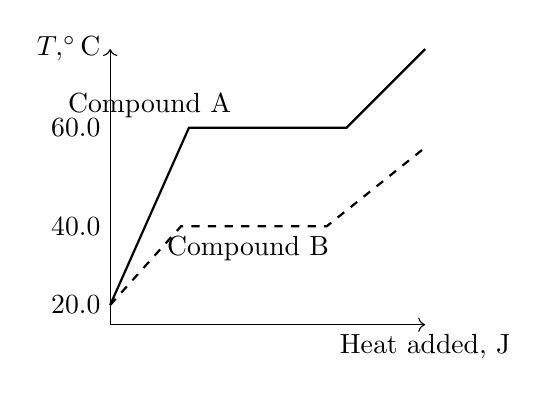
\begin{tikzpicture}[scale=0.5]
        \draw[->] (0,0) -- (8,0) node[below] {Heat added, J};
        \draw[->] (0,0) -- (0,7) node[left] {$T, ^\circ\text{C}$};
        \draw[thick] (0,0.5) -- (2,5) node[above, xshift=-0.5cm] {Compound A} -- (6,5) -- (8,7);
        \draw[thick, dashed] (0,0.5) -- (1.8,2.5) -- (5.5,2.5) node[below, xshift=-1cm] {Compound B} -- (8,4.5);
        \node[left] at (0,0.5) {20.0};
        \node[left] at (0,2.5) {40.0};
        \node[left] at (0,5) {60.0};
    \end{tikzpicture}
    \end{center}
    \begin{enumerate}
        \item The molar heat capacity of solid A is greater than that of solid B.
        \item The molar heat capacity of liquid A is greater than that of liquid B.
        \item The melting point of A is less than that of B.
        \item The heat of fusion of A is less than that of B.
    \end{enumerate}

    \item A sample of a pure substance is placed in a sealed, rigid container and the pressure is measured as a function of temperature. Which is the best explanation for the result shown?
    
    \begin{center}
    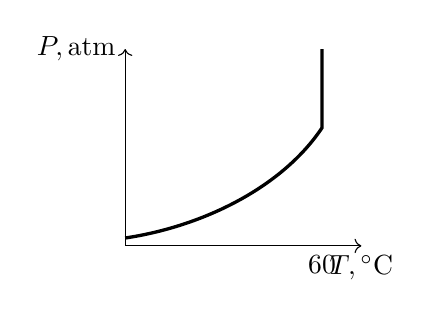
\begin{tikzpicture}[scale=0.5]
        \draw[->] (0,0) -- (6,0) node[below] {$T, {^\circ}\text{C}$};
        \draw[->] (0,0) -- (0,5) node[left] {$P, \text{atm}$};
        \draw[very thick] (0,0.2) .. controls (2,0.5) and (4,1.5) .. (5,3) -- (5,5);
        \node[below] at (5,0) {60};
    \end{tikzpicture}
    \end{center}
    \begin{enumerate}
        \item At lower temperatures, the substance is a mixture of solid and vapor, while at $60^\circ\text{C}$ the solid melts to give a mixture of liquid and vapor.
        \item At lower temperatures, the substance is a mixture of liquid and vapor, while at $60^\circ\text{C}$ only liquid is present.
        \item At lower temperatures, the substance is a mixture of liquid and vapor, while at $60^\circ\text{C}$ only a supercritical fluid is present.
        \item At lower temperatures, the substance consists of vapor only, while at $60^\circ\text{C}$ only a supercritical fluid is present.
    \end{enumerate}

    \item Cesium chloride ($M = 168.4$) crystallizes in a primitive cubic unit cell with each cesium ion surrounded by eight chloride ions arranged in a cube. The density of solid \ch{CsCl} is 3.988 g $\text{cm}^{-3}$. What is the Cs--Cl distance?
    \begin{enumerate}
        \item 206.2 pm
        \item 291.6 pm
        \item 357.1 pm
        \item 412.4 pm
    \end{enumerate}

    \item Steam turbines convert heat energy into mechanical work. Which statement best describes the efficiency of this process?
    \begin{enumerate}
        \item 100\%, because energy is conserved
        \item Less than 100\%, because the steam decreases in temperature
        \item Greater than 100\%, because the turbine increases in kinetic energy
        \item Can be greater than, less than, or equal to 100\% depending on the design of the turbine.
    \end{enumerate}

    \item At what temperatures is the decomposition of tungstic acid, \ch{H2WO4(s)}, to tungsten trioxide and water vapor spontaneous under standard conditions?
    \[ \ch{H2WO4(s) -> WO3(s) + H2O(g)} \]
    \begin{center}
    \small
    \begin{tabular}{ccc}
        Compound & $\Delta H^\circ_f, \text{kJ mol}^{-1}$ & $S^\circ, \text{J mol}^{-1}\text{K}^{-1}$ \\ \hline
        \ch{H2WO4(s)} & $-1130$ & $140$ \\
        \ch{WO3(s)} & $-840$ & $80$ \\
        \ch{H2O(g)} & $-240$ & $190$
    \end{tabular}
    \end{center}
    \begin{enumerate}
        \item $T > 385 \text{ K}$
        \item $T < 385 \text{ K}$
        \item The reaction is spontaneous at all temperatures.
        \item The reaction is not spontaneous at any temperature.
    \end{enumerate}

    \item In a well-insulated container, 10.0 g solid octane at its freezing point ($-56.9^\circ\text{C}$) is added to 300.0 mL liquid octane at $0.0^\circ\text{C}$ ($\text{density} = 0.71 \text{ g mL}^{-1}$). After equilibrium is achieved, the temperature is $-6.3^\circ\text{C}$. When the experiment is repeated under the same conditions except with 100.0 g solid octane, what is the final temperature?
    \begin{enumerate}
        \item $-39.7^\circ\text{C}$
        \item $-44.9^\circ\text{C}$
        \item $-51.7^\circ\text{C}$
        \item $-56.9^\circ\text{C}$
    \end{enumerate}

    \item Amphiphilic species like \ch{CH3(CH2)10COO-} can aggregate into micelles in water. $\Delta S$ for micelle formation is positive. Which best explains why?
    \begin{enumerate}
        \item Amphiphilic compounds are solvated by an ordered layer of water molecules.
        \item Micelle formation involves converting many independent amphiphilic compounds into a single large micelle.
        \item Water molecules are trapped in the hydrophobic interior of micelles.
        \item Water molecules form ordered structures around the exterior of micelles.
    \end{enumerate}

    \item What is $\Delta G^\circ_f$ of \ch{C2H4(g)} at $25^\circ\text{C}$?
    \begin{center}
    \small
    \begin{tabular}{ccc}
        Substance & $\Delta H^\circ_f, \text{kJ mol}^{-1}$ & $S^\circ, \text{J mol}^{-1}\text{K}^{-1}$ \\ \hline
        \ch{C2H4(g)} & $52.4$ & $219.3$ \\
        \ch{H2(g)} & $0$ & $130.7$ \\
        \ch{C(s, graphite)} & $0$ & $5.7$
    \end{tabular}
    \end{center}
    \begin{enumerate}
        \item $-13.0 \text{ kJ mol}^{-1}$
        \item $27.7 \text{ kJ mol}^{-1}$
        \item $46.9 \text{ kJ mol}^{-1}$
        \item $68.3 \text{ kJ mol}^{-1}$
    \end{enumerate}

    \item The $\Delta H^\circ_f$ of \ch{CH4(g)} is $-74.6 \text{ kJ mol}^{-1}$ and the bond dissociation enthalpies (BDEs) of several bonds are given:
    \begin{center}
    \small
    \begin{tabular}{cc}
        Bond & BDE, $\text{kJ mol}^{-1}$ \\ \hline
        \ch{C-C} & 347 \\
        \ch{C-H} & 413 \\
        \ch{H-H} & 432
    \end{tabular}
    \end{center}
    Based on these data, what is the molar enthalpy of sublimation of \ch{C(s, graphite)} to form \ch{C(g)}?
    \begin{enumerate}
        \item $713 \text{ kJ mol}^{-1}$
        \item $788 \text{ kJ mol}^{-1}$
        \item $1061 \text{ kJ mol}^{-1}$
        \item $1135 \text{ kJ mol}^{-1}$
    \end{enumerate}

    \item For a reaction $X + Y \rightarrow Z$, data for three experiments are given:
    \begin{center}
    \small
    \begin{tabular}{ccc}
        $[X]_0$, M & $[Y]_0$, M & Initial rate, $\text{M}^{-1}\text{min}^{-1}$ \\ \hline
        0.10 & 0.10 & $2.0 \times 10^{-4}$ \\
        0.30 & 0.10 & $6.0 \times 10^{-4}$ \\
        0.30 & 0.30 & $5.4 \times 10^{-3}$
    \end{tabular}
    \end{center}
    Which mechanism is consistent with the above data?
    \begin{enumerate}
        \item $\ch{2X <=> X2}$ (fast), $\ch{X2 + Y -> Z + X}$ (slow)
        \item $\ch{X + Y -> Z}$
        \item $\ch{2Y <=> Y2}$ (fast), $\ch{Y2 + X -> Z + Y}$ (slow)
        \item $\ch{X + Y <=> XY}$ (fast), $\ch{XY -> Z}$ (slow)
    \end{enumerate}

    \item $^{208}\text{Po}$ undergoes $\alpha$ decay to form stable $^{204}\text{Pb}$ with a half-life of 2.90 years. A sample of $^{208}\text{Po}$ was measured with a Geiger counter 5.20 years ago as having an activity of 1320 disintegrations per second. What is its activity today?
    \begin{enumerate}
        \item $137 \text{ s}^{-1}$
        \item $381 \text{ s}^{-1}$
        \item $736 \text{ s}^{-1}$
        \item $1320 \text{ s}^{-1}$
    \end{enumerate}

    \item A reversible reaction occurs as follows: $\ch{2A(g) + B(g) <=> C(g) + D(g)}$. Under a certain set of conditions, the rate law for the forward reaction is determined to be $\text{Rate} = k_f[A][B]$. Under these conditions, what is the rate law for the reverse reaction?
    \begin{enumerate}
        \item $\text{Rate} = k_r[C][D]$
        \item $\text{Rate} = \frac{k_r[C][D]}{[A]}$
        \item $\text{Rate} = \frac{k_r[C][D]}{[A]^2[B]}$
        \item It cannot be determined from the information given.
    \end{enumerate}

    \item A compound A reacts by two independent irreversible pathways to give two products, B and C. At 300 K, 35\% of the product is B, while at 320 K, 70\% of the product is B. What may be concluded about the activation energy of the pathway to form B compared to the activation energy of the pathway to form C?
    \begin{enumerate}
        \item The $E_a$ for the pathway to form B is higher by $28\text{ kJ mol}^{-1}$.
        \item The $E_a$ for the pathway to form B is higher by $59\text{ kJ mol}^{-1}$.
        \item The $E_a$ for the pathway to form B is lower by $28\text{ kJ mol}^{-1}$.
        \item The $E_a$ for the pathway to form B is lower by $59\text{ kJ mol}^{-1}$.
    \end{enumerate}

    \item The irreversible reaction $A + B \rightarrow C$ takes place by the following two-step mechanism involving an intermediate X whose concentration is low throughout the reaction:
    \[ \ch{A <=>[$k_1$][$k_{-1}$] X} \qquad \ch{X + B ->[$k_2$] C} \]
    Which statement cannot be correct regardless of the values of $k_1$, $k_{-1}$, and $k_2$?
    \begin{enumerate}
        \item The reaction is 0th order in A.
        \item The reaction is 1st order in A.
        \item The reaction is 0th order in B.
        \item The reaction is 1st order in B.
    \end{enumerate}

    \item Nitramide decomposes to nitrous oxide in aqueous solution: $\ch{NH2NO2(aq) -> N2O(g) + H2O(l)}$. In solutions with $\text{pH} \ge 12$, the rate law for this reaction is: $\text{Rate} = k\frac{[\ch{NH2NO2}]}{[\ch{H3O+}]}$. The reaction is monitored with $\text{pH} = 12.0$ (solid line) and with $\text{pH} = 12.3$ (dashed line). Which graph best represents the time-dependence of the nitramide concentrations?
    
    \begin{center}
    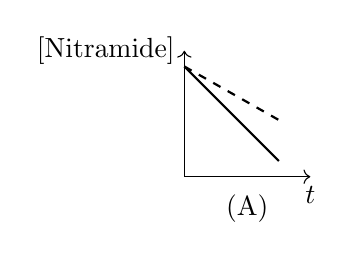
\begin{tikzpicture}[scale=0.4]
        \draw[->] (0,0) -- (4,0) node[below] {$t$};
        \draw[->] (0,0) -- (0,4) node[left] {$[\text{Nitramide}]$};
        \draw[thick] (0,3.5) -- (3,0.5);
        \draw[thick, dashed] (0,3.5) -- (3,1.8);
        \node at (2,-1) {(A)};
    \end{tikzpicture}
    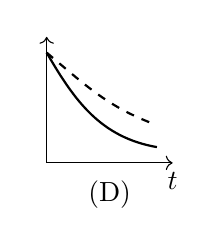
\begin{tikzpicture}[scale=0.4]
        \draw[->] (0,0) -- (4,0) node[below] {$t$};
        \draw[->] (0,0) -- (0,4) node[left] {};
        \draw[thick] (0,3.5) to[out=-60,in=170] (3.5,0.5);
        \draw[thick, dashed] (0,3.5) to[out=-40,in=160] (3.5,1.2);
        \node at (2,-1) {(D)};
    \end{tikzpicture}
    \end{center}
    \begin{enumerate}
        \item (A)
        \item (B)
        \item (C)
        \item (D)
    \end{enumerate}

    \item A sample of 0.320 mol of a weak monoprotic acid in 1.00 L of solution is 10.2\% ionized. What is $K_a$ for this acid?
    \begin{enumerate}
        \item $3.3 \times 10^{-3}$
        \item $3.7 \times 10^{-3}$
        \item $3.2 \times 10^{-2}$
        \item $1.1 \times 10^{-1}$
    \end{enumerate}

    \item Typically, the molar solubility $x$ of an ionic compound in pure water and its $K_{sp}$ are related by a simple formula. Which formula is not expected for $K_{sp}$ for an ionic compound?
    \begin{enumerate}
        \item $K_{sp} = 4x^3$
        \item $K_{sp} = 4x^4$
        \item $K_{sp} = 27x^4$
        \item $K_{sp} = 81x^5$
    \end{enumerate}

    \item Equal volumes of 0.1 M solutions of \ch{NaH2PO4} and \ch{Na3PO4} are mixed. What is the pH of the resulting solution? For \ch{H3PO4}, $pK_{a1} = 2.12$, $pK_{a2} = 7.21$, $pK_{a3} = 12.32$.
    \begin{enumerate}
        \item 4.66
        \item 6.66
        \item 7.21
        \item 9.76
    \end{enumerate}

    \item 5.00 g of nitrogen dioxide is introduced into an evacuated, rigid 1.00 L container. It is allowed to equilibrate according to the reaction below at 310 K, and the total pressure in the vessel is 1.71 bar. What is $K_p$ for the reaction at 310 K?
    \[ \ch{N2O4(g) <=> 2NO2(g)} \]
    \begin{enumerate}
        \item 0.35
        \item 0.57
        \item 2.28
        \item 2.92
    \end{enumerate}

    \item A mixture containing \ch{CO(g)}, \ch{H2O(g)}, \ch{CO2(g)}, and \ch{H2(g)} is allowed to reach equilibrium at $120^\circ\text{C}$ in a container that maintains a constant total pressure of 1.0 bar.
    \[ \ch{CO(g) + H2O(g) <=> CO2(g) + H2(g)} \]
    5.0 g of \ch{H2O} is added to this container, which is allowed to reattain equilibrium (still at $120^\circ\text{C}$ and 1 bar total pressure). How does the partial pressure of \ch{H2(g)} change as a result of the addition of \ch{H2O}?
    \begin{enumerate}
        \item The partial pressure of \ch{H2(g)} increases.
        \item The partial pressure of \ch{H2(g)} decreases.
        \item The partial pressure of \ch{H2(g)} does not change.
        \item The effect on the partial pressure of \ch{H2(g)} cannot be determined from the information given.
    \end{enumerate}

    \item 0.01 mol of \ch{AgNO3} is dissolved in 1.00 L of 1.00 M aqueous \ch{NH3}. What is the minimum amount of \ch{HCl} that would need to be added to this solution to induce precipitation of \ch{AgCl}? The $K_{sp}$ of \ch{AgCl} is $1.8 \times 10^{-10}$; the $K_f$ of \ch{Ag(NH3)2+} is $1.6 \times 10^7$ and the $K_a$ of \ch{NH4+} is $5.6 \times 10^{-10}$.
    \begin{enumerate}
        \item $1.8 \times 10^{-8} \text{ mol}$
        \item $1.3 \times 10^{-5} \text{ mol}$
        \item $0.18 \text{ mol}$
        \item $0.28 \text{ mol}$
    \end{enumerate}

    \item In which compound does the oxidation number of oxygen differ from $-2$?
    \begin{enumerate}
        \item \ch{NaBO3}
        \item \ch{NaNO3}
        \item \ch{K3PO4}
        \item \ch{K2Cr2O7}
    \end{enumerate}

    \item Copper metal reacts with nitric acid to form \ch{NO(g)} as shown in the unbalanced reaction shown below. When the reaction is balanced using lowest whole number coefficients, what is the coefficient of \ch{H+(aq)}?
    \[ \ch{Cu(s) + H+(aq) + NO3-(aq) -> Cu^2+(aq) + NO(g) + H2O(l)} \]
    \begin{enumerate}
        \item 2
        \item 4
        \item 6
        \item 8
    \end{enumerate}

    \item In the Hall--Héroult process for producing aluminum, aluminum is electrolytically reduced from \ch{Al2O3} dissolved in molten cryolite, \ch{Na3AlF6}, while a graphite anode is oxidized to \ch{CO2}. What is the ratio of the mass of Al deposited on the cathode to the mass of C lost from the anode?
    \begin{enumerate}
        \item 1.50:1
        \item 2.25:1
        \item 3.00:1
        \item 3.36:1
    \end{enumerate}

    \item The cathode of an electrolytic cell with a copper electrode initially has 100.0 mL of a solution that is 1.00 M in both \ch{Cu^2+(aq)} and \ch{Fe(CN)6^3-(aq)}. The solution is electrolyzed with a constant current of 0.500 A at a constant temperature of 298 K. How much time elapses before \ch{Cu(s)} begins to deposit on the electrode?
    \begin{center}
    \small
    \begin{tabular}{cc}
        Half-reaction & $E^\circ$, V \\ \hline
        \ch{Fe(CN)6^3-(aq) + e- -> Fe(CN)6^4-(aq)} & 0.370 \\
        \ch{Cu^2+(aq) + 2e- -> Cu(s)} & 0.337
    \end{tabular}
    \end{center}
    \begin{enumerate}
        \item 0 min
        \item 89.4 min
        \item 252 min
        \item 322 min
    \end{enumerate}

    \item A molecule absorbs a photon of light to form an excited state. How do the redox properties of the excited state compare to those of the ground state?
    \begin{enumerate}
        \item The excited state is both a stronger oxidizing agent and a stronger reducing agent than the ground state.
        \item The excited state is both a weaker oxidizing agent and a weaker reducing agent than the ground state.
        \item The excited state is a stronger oxidizing agent but a weaker reducing agent than the ground state.
        \item The excited state is a weaker oxidizing agent but a stronger reducing agent than the ground state.
    \end{enumerate}

    \item What is $\Delta G^\circ$ at 298 K for the disproportionation of \ch{PbO(s)}?
    \[ \ch{2PbO(s) -> PbO2(s) + Pb(s)} \]
    \begin{center}
    \small
    \begin{tabular}{cc}
        Half-reaction & $E^\circ$, V \\ \hline
        \ch{PbO2(s) + 4H+(aq) + 4e- -> Pb(s) + 2H2O(l)} & 0.671 \\
        \ch{PbO(s) + H2O(l) + 2e- -> Pb(s) + 2OH-(aq)} & $-0.580$
    \end{tabular}
    \end{center}
    \begin{enumerate}
        \item $163 \text{ kJ mol}^{-1}$
        \item $241 \text{ kJ mol}^{-1}$
        \item $403 \text{ kJ mol}^{-1}$
        \item $483 \text{ kJ mol}^{-1}$
    \end{enumerate}

    \item For which gas-phase atoms is addition of an electron endothermic?
    \[ \text{I. Li} \qquad \text{II. Ne} \]
    \begin{enumerate}
        \item I only
        \item II only
        \item Both I and II
        \item Neither I nor II
    \end{enumerate}

    \item Which atom has the lowest first ionization energy?
    \begin{enumerate}
        \item Be
        \item B
        \item Mg
        \item Al
    \end{enumerate}

    \item How many electrons in a ground-state gas-phase atom of arsenic (As) have a quantum number $m_l = 1$?
    \begin{enumerate}
        \item 5
        \item 7
        \item 15
        \item 18
    \end{enumerate}

    \item Which orbital has the same number of radial nodes as a 3s orbital?
    \begin{enumerate}
        \item 3p
        \item 4s
        \item 4f
        \item 5d
    \end{enumerate}

    \item Which lanthanide has a common oxidation number different from +3?
    \begin{enumerate}
        \item Ce
        \item Gd
        \item Er
        \item Lu
    \end{enumerate}

    \item Which radioisotope decays by beta ($\beta^-$) emission?
    \begin{enumerate}
        \item $^{20}\text{Na}$
        \item $^{52}\text{V}$
        \item $^{54}\text{Co}$
        \item $^{62}\text{Cu}$
    \end{enumerate}

    \item Which is a valid Lewis structure for nitric acid, \ch{HNO3}?
    \begin{enumerate}
        \item \chemfig{H-O-N(=[2]O)-O^{-}}
        \item \chemfig{H-N(=[2]O)(-[4]O)-O}
        \item \chemfig{H-O-N(=[2]O)=O}
        \item \chemfig{H-O-O-N=O}
    \end{enumerate}

    \item Which statements about carbon--oxygen bond lengths are correct?
    \begin{itemize}
        \item[I.] The carbon--oxygen bond in carbon dioxide, \ch{CO2}, is shorter than the carbon--oxygen bond in carbonyl sulfide, \ch{COS}.
        \item[II.] The carbon--oxygen bond in phosgene, \ch{COCl2}, is shorter than the carbon--oxygen bond in urea, \ch{CO(NH2)2}.
    \end{itemize}
    \begin{enumerate}
        \item I only
        \item II only
        \item Both I and II
        \item Neither I nor II
    \end{enumerate}

    \item Which statement best describes the relative Lewis acidity of \ch{BF3} and \ch{BCl3}?
    \begin{enumerate}
        \item \ch{BF3} is a weaker Lewis acid than \ch{BCl3} because F is more electronegative than Cl.
        \item \ch{BF3} is a weaker Lewis acid than \ch{BCl3} because F is a better $\pi$ donor than Cl.
        \item \ch{BF3} is a stronger Lewis acid than \ch{BCl3} because F is more electronegative than Cl.
        \item \ch{BF3} is a stronger Lewis acid than \ch{BCl3} because F is a better $\pi$ donor than Cl.
    \end{enumerate}

    \item Which comparisons of bond angles are correct?
    \begin{itemize}
        \item[I.] The bond angle in \ch{NH3} is greater than the bond angle in \ch{NF3}.
        \item[II.] The bond angle in \ch{NH3} is greater than the bond angle in \ch{PH3}.
    \end{itemize}
    \begin{enumerate}
        \item I only
        \item II only
        \item Both I and II
        \item Neither I nor II
    \end{enumerate}

    \item The gas-phase molecules \ch{B2} and \ch{O2} are both paramagnetic. Which statement about the relative energies of their molecular orbitals explains these observations?
    \begin{itemize}
        \item[I.] The $\sigma_{2p}$ MO is higher in energy than the $\pi_{2p}$ MOs.
        \item[II.] The $\sigma^*_{2p}$ MO is higher in energy than the $\pi^*_{2p}$ MOs.
    \end{itemize}
    \begin{enumerate}
        \item I for \ch{B2}, II for \ch{O2}
        \item I for \ch{O2}, II for \ch{B2}
        \item I for both \ch{B2} and \ch{O2}
        \item II for both \ch{B2} and \ch{O2}
    \end{enumerate}

    \item How many stereoisomers are there of the octahedral coordination complex $[\ch{Co(NH2CH2CO2)3}]$?
    \begin{enumerate}
        \item 1
        \item 2
        \item 3
        \item 4
    \end{enumerate}

    \item How many tertiary alcohols have the formula \ch{C5H12O}?
    \begin{enumerate}
        \item 1
        \item 2
        \item 3
        \item 4
    \end{enumerate}

    \item Which difluorocyclohexanes are optically active?
    \begin{center}
        I. \text{trans-1,2-difluorocyclohexane} \qquad II. \text{cis-1,3-difluorocyclohexane}
    \end{center}
    \begin{enumerate}
        \item I only
        \item II only
        \item Both I and II
        \item Neither I nor II
    \end{enumerate}

    \item Which best describes the outcome of extracting a dilute solution of benzoic acid in diethyl ether with 5\% aqueous \ch{NaHCO3}?
    \begin{enumerate}
        \item Benzoic acid is present in the bottom layer.
        \item Benzoate ion is present in the bottom layer.
        \item Benzoic acid is present in the top layer.
        \item Benzoate ion is present in the top layer.
    \end{enumerate}

    \item Which product would be obtained in the greatest quantity from bromination of 4-nitrotoluene using an aluminum bromide catalyst?
    \begin{center}
        \chemfig{*6(-(-CH_3)=--(-NO_2)=--)} \quad $\xrightarrow{\ch{Br2}, \ch{AlBr3}}$
    \end{center}
    \begin{enumerate}
        \item 2-bromo-4-nitrotoluene
        \item 3-bromo-4-nitrotoluene
        \item 2,6-dibromo-4-nitrotoluene
        \item 3,5-dibromo-4-nitrotoluene
    \end{enumerate}

    \item Which compound is least reactive toward ethylmagnesium bromide, \ch{CH3CH2MgBr}?
    \begin{enumerate}
        \item \chemfig{CH_3-CH_2-CHO}
        \item \chemfig{CH_3-CO-CH_3}
        \item \chemfig{CH_3-CH_2-COOCH_3}
        \item \chemfig{CH_3-CH_2-COCH_2-CH_3}
    \end{enumerate}

    \item Which statements describe significant differences between RNA and DNA?
    \begin{itemize}
        \item[I.] The bases used in RNA include three purines and one pyrimidine, while those in DNA include two purines and two pyrimidines.
        \item[II.] Hydrolysis of RNA frequently involves cyclic phosphate intermediates, while hydrolysis of DNA never does.
    \end{itemize}
    \begin{enumerate}
        \item I only
        \item II only
        \item Both I and II
        \item Neither I nor II
    \end{enumerate}

\end{enumerate}

\end{document}